\documentclass[11pt]{article}

\usepackage{fullpage}
%\usepackage{newcent}  % times, palatino, newcent and bookman
\usepackage{bera}   % install texlive-fonts-extra for Bera fonts. Good for
                    %  non-printout reading
%\usepackage{enumitem}   % bullet point customization. Needed for Droid and DejaVu fonts
                         %  Add [label=$\bullet$] for itemize headings.
\usepackage{hyperref}
\usepackage{dtklogos}   % for \BibTeX

\usepackage{graphicx}   % for jpg image import

\begin{document}

\section{Introduction}

Writing a Ph.D. dissertation is a daunting task. But my experience was not
that extremely hard; for my case, the hard part was not with the writing, but
with managing the research process. This was actually much, much harder than I
had expected --- and I heard similar things from my friends who had already
got their Ph.D. degrees ahead of me.

But for writing part, believe me --- it can be \emph{strangely} fun.  Writing
is a great process that conveys your thinking to other people.  Of course
there are other ways to express your thinkings; presentations, discussions,
lectures, and so on.  However, the point of writing is that it is like a
construction process that eventually leads to a \emph{great} building.  If I
rely on analogy, presentations and lectures are like creating small rooms and
facilities \emph{inside} your building. Only writing can connect and organize
them into a huge, great-looking skyscraper.

In this manuscript, I intend to lay out my lessons writing my Ph.D.
dissertation. Well, I do not think that my writing, especially my
dissertation, is a quality one. But my writing experience has been felt great
most of time. And I want to share my experience --- particularly in terms of
what you need to prepare --- with other ABD\footnote{Informal acronym for
all-but-dissertation} students out there. In addition, I want to talk about good
tools out there for dissertation writing.  Different people use different
tools but the technical advances in ``writing support'' have been amazing to
me during my dissertation writing.  Be sure to get the benefit out of them.

\subsection{Other guides and tutorials}
There are a bunch of them. Some popular ones are:

\begin{itemize}
    \item Tomorrow's Professor: Preparing for Careers in Science and
        Engineering

        This book is a classic. Actually, I did not buy this book for the
        simple reason of being-too-expensive. Instead, I 
        subscribed for an e-mail list which turned out to be pretty helpful. 
        Check out the link at
        \begin{small}\url{http://cgi.stanford.edu/\~dept-ctl/cgi-bin/tomprof/postings.php}.\end{small}

    \item Getting What You Came For: The Smart Student's Guide to Earning an
        M.A. or a Ph.D.

        This is another great book for any graduate students, particularly for
        Ph.D. students. I hear a lot of good praises about this book from my
        colleagues too. Personally, one problem was that I had not quite fully
        understood what the book was actually talking about \emph{before} I
        met the situation myself and went it through (for example,
        explanations on the experience examples for a comprehensive exam). 

        Still, well, it is definitely better than tackling something without
        knowing anything at all. So keep a copy near you.

\end{itemize}


\section{Thoughts and tips for writing}

\subsection{Write regularly, but not that much}
One thing you will realize after you are done with your first dissertation
draft --- is probably that you have been writing one page per day on average
(double-spaced, 12 pt.).

But please note that this measure is ``on average''. Sometimes you might be
writing a lot, with your fingers gliding smoothly over the keyboard.  Of
course some other times you might be looking at the blinking cursor for hours
and hours without typing anything at all. 

The point of writing, in my opinion, is to realize that this is a mental
process of pouring down the flow of your thought into a organized form.  And
like it or not, your mental process is dominated by your cognitive state at
this moment. First comes your subconsciousness. You cannot control it but
somehow you will notice that your subconsciousness plays a big part with your
writing performance; sometimes you have a lot of thoughts but sometimes not.
This is because not all of your thoughts are created from your consciousness.
If your subconsciousness is not feeling well, you will be facing a strange
paucity in the amount of any thoughts in your brain.

Therefore, you cannot avoid writing almost nothing when you do not have any
thoughts to write. This is actually very natural; when there is almost nothing
in your brain, stop writing. Do something else. A good news is that your
subconsciousness is still working even when you are sleeping.  When your
subconsciousness creates sufficient amount of thoughts, you will be naturally
writing a lot. 

Second, your thoughts have water-like streaming characteristics.  They are not
like a stack of materials stored inside a closet, as we typically imagine.
When your thought comes up, you need to ``save'' it somewhere because it is
flowing and going away soon.  Of course you can retrieve it from your memory
later, but a lot of time it is hard since it requires a queue (or a key as in
a key-value pair in computer science) to access the stored memory.

For this reason, when thoughts are coming up, try best not to let them flow
away. Sit down and write --- at least several words (which can be a queue for
easily retrieving all the thoughts you are having right now). If you don't
have computers nearby, use a pencil and a piece of paper. 

And a habit of writing down right at the moment when thoughts are coming up
helps the current flow keep going. This is important. If the stream dries up
completely, you will be having a hard time taking the water from deep down the
well of ideas.  But if you keep writing --- not too frequently but sufficient
enough to keep a very shallow thought stream --- then your brain will keep
rollin' on.

So the point is that you do not stop writing completely, especially for a long
time like a week or so.\footnote{This can be different when you
    are writing a paper instead. For paper writing, a process of ``stop
    writing for fermentation'' can be helpful to upgrade your work into a
quality one, as if fermentation transforms milk into tasty cheese. Refer to
Varian~\cite{varian-building-model} for more information} If writing your dissertation feels like
too stressful, work on ``writing'' something else. Keep your brain warmed up
--- but just enough to avoid complete freezing. 

\subsubsection{Working hard for writing?}

However, sometimes, actually more than frequently, your brain needs a break.
If you observe yourself carefully, you will see that your writing performance
pattern shows a lot of fluctuations even for a day. One strange thing is that
your brain needs a lot of energy to work on writing. The brain can be
energized only when you have (i) sufficient amount of quality food \emph{and}
(ii) a lot, lot, lot of break (such as sleeping). 

So working up too late and getting up early to meet other schedules is not a
good strategy when you need to write some important things. From my
experience, it was better to sleep say, for 10 hours, and efficiently work on
my writing for two hours, than to trying hard to write something for 6 hours
after getting 6 hours of sleep. 

And another strange thing is that you need a get-away break sometimes to keep
your brain fresh. What you notice at this point is that you actually cannot
write anything. And you will probably see that you cannot do other things
easily as well and even reading a gossip story about a celebrity will feel like
a burden. Then you do need a reboot as you do sometimes with your computer.
For me, if I keep thinking about driving four hours to New Jersey for a Korean
hot spa trip, then it is usually time for a ``reboot'' myself. 

But most students, including me, make a poor decision of working harder and
harder to overcome this situation. Well, it might be needed for a military
exercise where a failure might mean life or death, but this only make the
situation worse when you work on research. Even in a military setting, I think
generals planning strategies must sleep sufficiently. That's the way brain
works. 

% on average, you will find that you write one page (double-spaced, 12
% pt.) per day for your dissertation.

\subsubsection{Write some other stuffs}
% Writing takes a lot of practice time.
Unfortunately, becoming a \emph{good writer} takes a long time. I need more
time to become a good writer too. As an international student with English
being my second language, it is much harder for me than my English-speaking
colleagues. To make matters worse, the Korean language is quite different from
English in every aspects; a lot of time I envy my Chinese colleagues because
Chinese is way much closer to English in terms of grammar, not to mention
people from countries speaking Indo-european languages.

But what writing actually requires, especially academic writing, is your
reasoning skill, not much as language skills. Training your brain into
generating a stream of well-organized reasoning thoughts takes a huge amount
of time. 10,000 hours? [CITE]

Therefore, write something all the time. Anything is fine. Diary, notes,
e-mails, and so on. But one of the best writing practice can be keeping an
online blog. Blog postings are typically longer than other form of online
writing and this is the environment that induces your brain to organize your
thoughts. 

In addition, reading books can be important too. Creativity usually starts
with imitation. When you read a lot, you will have raw materials for better
writing.  When you want to take a break, feel free to read. For academic
writers, reading is actually another form of writing practice.

\subsection{Writing in some other forms}
Some of my friends are actually very good at this. They use Powerpoint slides
extensively --- like writing down your thoughts, ideas, titles of nice articles,
etc. onto PowerPoint, rather than using a word processor or other note-taking
applications such as Evernote or OneNote.

The advantage of this is twofolds: first, laying out bullet-points is usually
easier than writing sentences or paragraphs. Second, you can save time
creating your presentation slides with these Powerpoint-based notes. Since the
flow of your thought is important with your presentation, writing ``thoughts''
directly down in the form of slides are actually helpful for your future oral
presentation --- and easier than creating presentation slides after going over
your paper (which has to include a reorganization process of your thoughts).

Interestingly, this was not working very well for me; I guess this is due to
my personal characteristic, but the \emph{idea} of laying out bullet-points
worked with when I was doing my literature review. When I found out several
interesting articles, I usually open up Microsoft OneNote window and start
writing down with bullet-points using indents.(You might use word processors
or other tools as well)

I do not put much there. Just some keywords or my thoughts with several words
or a sentence at maximum. When I am done with this, I just leave it there.
When it comes down to writing a literature review part of my paper, this
expedites my writing process; I just take one line or two and convert it into
sentences.

So this switching between bullet-points and formal sentences/paragraphs helps
my writing process in two ways. First, it makes my finger keep typing. Second,
it makes easier for me to build nice sentences later --- from pieces of a
few words.

I still think the PPT note-taking idea from my friend is effective. However,
you might want to transform it a little bit to suit your style and needs. And
remember that bullet-type writing is usually easier even when you are stuck
and cannot write a single sentence at all.

\subsection{Work smart, not hard}

You do not want it and I do not like it either. But put the highest priority
on your writing work from your to-do-list for today. Only when your brain is
fresh, you can write. When you start your work, get the writing done first and
do other things later. Even a small bit of fatigue in your brain will
greatly hamper your writing performance. And be sure to get a lot of sleep.

\subsection{Separate writing and editing}
One legendary(?) tip coming from so-called ``prolific'' writers is
that you need to separate writing from editing when you want to write
a lot. It sounds simple. And it was not actually that hard when I
was practicing it either. Dump whatever thoughts you have right now.
Minimize hitting on backspace key. Of course do not think about grammars
or whatever. Forget about it after done with dumping. Get a good sleep.
Then do editing tomorrow.

The main advantage of this separation technique is that you can save a lot of
materials that otherwise would have been cut and discarded by your editing
thought process inside your brain. Simply storing the thoughts in the form of
sentences help stacking up the materials.  Storing them inside your brain in
the form of thoughts are susceptible to volatility.

[But what was the problem with this technique??? Drafter/planner tradeoff?]
[Write more on the side-effect of ``writing too much'']

\section{Tools}

\subsection{LaTeX}
No wonder LaTeX takes care of numerous chores in dissertation writing for you.
For example, you no longer need to pay attentions to the layout of the
figures.  Table of Contents is automatically generated, and the numbering for
tables, figures, math equations, theorems, and so on are all automatically
taken care of. 

But the most significant feature of LaTeX, in terms of researchers'
perspective, is its citation management combined with BibTeX. A researcher has
to know \emph{where} his knowledge comes from and that is the reason why we
need to keep it a habit of tracking citation records.  The number of citations
for a Ph.D. dissertation easily surpasses 100.  If you do not do the record
keeping, you will be always lost in recovering your memory.

So how does BibTeX manage your citation records? BibTeX citation file is a
simple text file with specific citation field records (See
Fig.~\ref{fig:bibtex-example} for an example). You just need to add entries
whenever you come across any good papers. 

There are other alternatives such as EndNote. EndNote is popular with
Microsoft Office users. I do not have any experience with EndNote, so I skip
EndNote in this manuscript. 

\begin{figure}[ht]
    \begin{center}
    \begin{footnotesize}
\begin{verbatim}
@ARTICLE{gode-sunder-1993,
  author = {Gode, Dhananjay K. and Sunder, Shyam},
  title = {Allocative Efficiency of Markets with Zero-Intelligence Traders:
    Market as a Partial Substitute for Individual Rationality},
  journal = {Journal of Political Economy},
  year = {1994},
  volume = {101},
  pages = {119--137}, 
  number = {1},
  month = feb,
  issn = {0022--3808},
  shorttitle = {Allocative Efficiency of Markets with Zero-Intelligence Traders},
  abstract = {},
  url = {http://www.jstor.org/stable/2138676}
}
\end{verbatim}
    \end{footnotesize}
    \end{center}
    \caption{A \BibTeX~entry example for a journal paper.}
    \label{fig:bibtex-example}
\end{figure}


\subsubsection{A process of building and managing your paper collection}
Personally, I recommend using the combination of Zotero, BibTeX (and LaTeX of
course) for managing your paper collection. Imagine it like managing your MP3
music collections. How do you manage your music collection with, say, iTunes
or Google Music? You download or purchase MP3 files of your choice, store them
into iTunes folders or Google Music cloud space. Whenever you want to listen
to them, you rely on browsing or searching features from your iTunes or Google
Music.

Similar process can be true of your academic paper collections. Think of
Zotero as the iTunes for your paper collection. You search for a paper and
download it. Then you save it to Zotero so that Zotero can automatically add
the paper to your collections. 

Similar to that iTunes can detect the MP3 tags with artist name, song title,
album title, etc., Zotero can automatically detect the paper title, author
names, published journal or conference name, publication date, and so on. If
Zotero fails to autodetect, you can manually enter the information too.

But you need to \emph{export} your Zotero collection into a BibTeX format
text file in order to include the citations as inline ones for your
dissertation. This is a step not needed for MP3 collections. You just pick one
MP3 file and listen to it. For paper writing, imagine like you are writing a
MP3 playlist. But the playlist for your paper has to have an intermediary
format and BibTeX is the format for the papers being written in LaTeX.

What is the advantage of having another BibTeX format? One handy feature is
that academic paper search services such as Google Scholar or Elsvier provide
the citation information in BibTeX format. You can export from Zotero. But you
do not necessarily do it from Zotero and you are not locked-in the Zotero
service only. 

[some conclusive remarks?]

\paragraph{Managing paper pdf files}
This section is my praise for Zotero; when you search for a paper and
save the web page to Zotero service, Zotero not only saves the web page
but also stores the paper pdf files automatically. This saves you a lot
of effort from keeping two separate collections simultaneously: citation
database and paper PDF file database.

This feature is very simliar to Evernote's. Whenever you click on the Evernote
button from your web browser, the Evernote plugin clips your web page of
interest and saves it. Zotero does the same but it automatically recognizes
the paper PDF file linked on the web page and save them altogether, 
generating a catalogue.

\subsection{Editors for LaTeX writing}

There are a bunch of them --- basically you can use Windows Notepad as well.
But having a LaTeX-aware provides a great boost with your work efficiency. For
me, I find syntax highlighting (or coloring), auto indentation, and auto
word-completion (citations, links, etc)  features helpful. Note that these
features are all present for any LaTeX editors.

One thing I would like to recommend to you writers is so-called
``distraction-free'' feature. A number of editors have this --- it creates a
full-screen editing environment, without a pull-down menus or icons for other
jobs that might distract you into something else. Please have a look at my
working environment (Fig.~\ref{fig:distraction-free}):

\begin{figure}[h]
    \begin{center}
        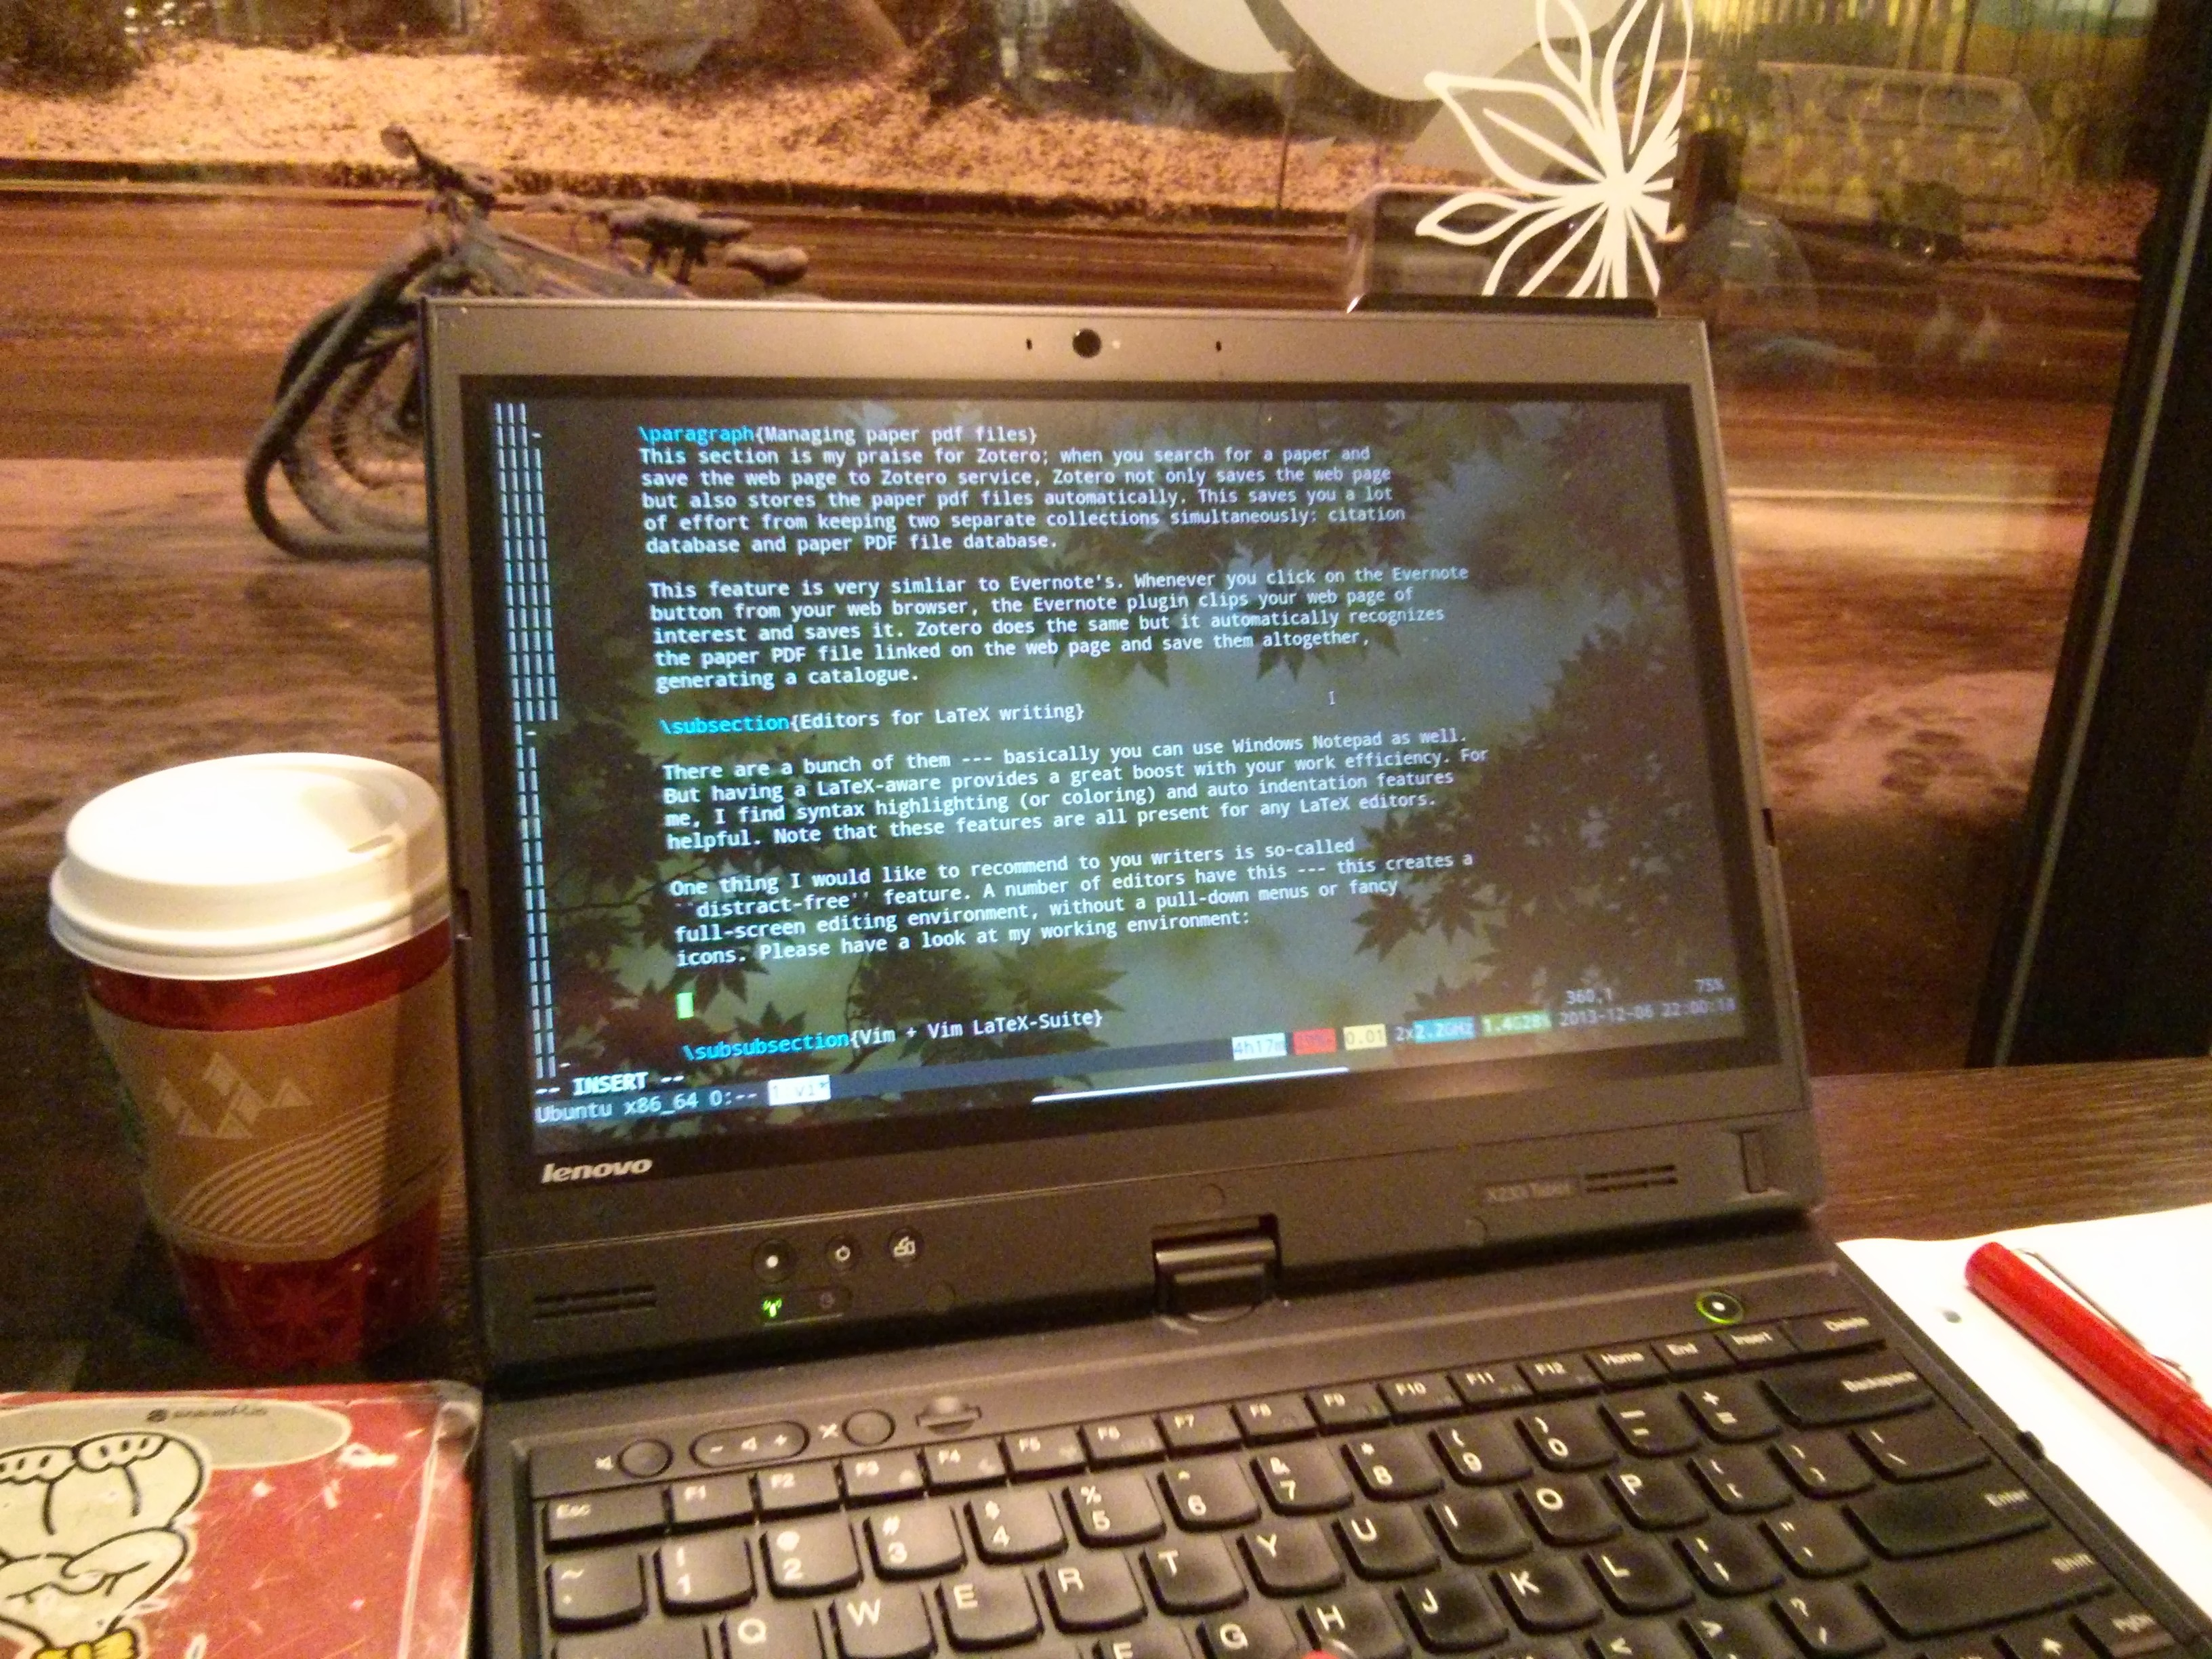
\includegraphics[width=0.7\textwidth]{figure/distract-free-shot}
    \end{center}
    \caption{A ``distraction-free'' editing with \texttt{vim} on a Linux
        terminal}
    \label{fig:distraction-free}
\end{figure}

See? This helps you with not wasting time your away with clicking on here and
there on your web browser. 

\subsubsection{TeXMaker, TeXShop on Mac, and TeXTronics}
If you think you are a beginner, start with TeXMaker. You won't regret it. If
you are a Mac enthusiast, consider TeXShop as well. However, note that
TeXMaker is cross-platform; it runs on Windows, Mac OS X, and Linux as well.

Some people recommend TeXTronics but I am not so sure about its advantages.

\subsubsection{Sublime Text 2 or 3}
People are raving on it. Seriously. This is an editor that you might want to
purchase. 

One drawback is that Sublime Text needs customizations. It is a
general-purpose editor, not only for writing LaTeX documents, but also for
writing in other programming languages such as C, Java, Python, Ruby, etc.
However, once setup, Sublime Text becomes very handy and user-friendly. 

In addition, Sublime Text is highly configurable. Therefore you can customize
it at your will: font and paragraph customization, themes, shortcut keys,
distraction-free environment, preview mode, 80-column indicator, and so on. 
Some people say that this is the editor with emacs-level configurability.
And there are tons of 3rd-party plug-ins. 

Sublime Text is the best editor I would like to recommend, if I have to choose
one from this section (and TeXMaker as the second for its ease of use). Be
sure to give it a serious try at least once.

\subsubsection{Vim + Vim LaTeX-Suite}
This is my personal choice but learning \texttt{vi} can be a pain when you are
not accustomed to Linux or shell environment. In other words, very nice for
geeks but not very recommended for other users. (And you probably know by now
if you need to skip this section or read further.)

In case you are using \texttt{vim}, be sure to have a serious look at Vim
LaTeX-Suite. \texttt{vim} is good enough, but LaTeX-Suite is a plug-in for
\texttt{vim} and provides extra features such as paragraph folding and quick
search for your BibTeX entries. 

Of course, you can use the holy \texttt{emacs} instead of \texttt{vim}.
\texttt{emacs} is always rich with great features that human minds can
ever imagine. 

One clear disadvantage with \texttt{vim} is its multi-window support.
\texttt{vim} is now equipped with multi-window support, but my opinion is that
\texttt{vi}'s interface is not very much multi-window friendly. For me, I
ended up using \texttt{byobu}, which is an enhancement on the classic
\texttt{screen}. Or you can use any terminal emulator with multiple tab-window
support.

When you use \texttt{byobu}, some shortcut keys conflict with Vim
LaTeX-Suite's. A quick tip: press \texttt{shift + F12} key to disable them.

\subsubsection{Online LaTeX editors:}

Templates available. Especially resume or CV's.

\subsubsection{Fixed-width fonts}

Better fonts than Courier new.

\subsection{Learning LaTeX}

Math on LaTeX.

StackExchange is awesome.

\subsection{Packages}

AMSmath and AMSsymb packages: indispensable.

Some font packages: But use Computer Modern for printouts. On screen: CM is
not good. Use up-to-date fonts: 

fullpage

setspace: onehalfspacing, doublespacing

\subsubsection{Tables, Figures, and picture import}

start from \\includegraphics.

Tables and Figures: Use this template.

Pictures: use png most of time. pdf is actually better in terms of
high-resolution printing. Note that MS Office now provides save-as-pdf feature
as well. 

Look for conferences or journals: they have nice templates as well.


\subsubsection{Creating a poster with LaTeX}

pros: Scales easily. Flexible textbox support. Math equations

cons: Takes more time for learning than using ppt. 

poster tips: 24in by 36in is a US standard. 3-fold poster panel size: 48in by
36in. Most large-format printers support up to 42in.

Cheapest one: use Acrobat reader and color print with the poster option.
Letter-sized mosaics. Glue them on the poster panel. 

Tips for using Sans Serif fonts: \\usepackage. Droid, Dejavu, Bera, Helvet,
etc. Sans Serif fonts are good for ppts or presentation materials. Complaints
about Arial. Microsoft's C-series fonts are pretty good but limited use under
LaTeX environment.



\section{Mental support}

\subsection{Counselling}
It might sound strange, but this can be important for your research.
Sometimes you can have difficult time making progress as a researcher due to
some emotional factors. If this is so, consider talking to a counsellor.
Usually the symptoms for any emotional problems for a Ph.D.  program student
can be roughly referred to ``depressions.'' However, there are numerous
reasons when a person experiences depression and it is often hard to identify
the specific cause for the depression.

Counsellors are professionals trained to detect this specific cause of the
depression and they can give you ``prescriptions'' depending on your specific
type of the depression identified. For example, some people have trouble with
fear management. Others might have problems with concentration. These are
beyond the scope of your advisor --- actually way up beyond their handling
capability.

One tip is that you probably have health insurance coverage for counselling. A
good(?) news is that the coverage for counselling is usually very nice when
your insurance coverage comes from your graduate assistantship work. (TA or
RA) So use them if you need --- not only for your mental health but also for
your research output --- and work efficiency including your advisor and
your department as a big community.

\section{Fun, hobby work}

One thing I regret is that I have not had any hobby (or fun) work during my
long Ph.D. program period --- note that I use the word ``hobby work'' instead
of ``hobby'' or just ``fun.'' Do it. Do it regularly like a work --- or do it
like a regular exercise or training depending on your personal taste.

The main reason is that (again!) your brain does need breaks. Having a break
from your research work is hard since it is a mental process. As long as you
are awake, some thoughts on your research work will always pop up. Well,
sometimes you will see them in your dream as well. 
%So it is extremely hard to let your brain --- which is the engine for your
%research work --- have some break.

So you have to figure out a way to \emph{enforce} some regular break to your
brain. The easiest way is to make your brain concentrate on a totally
different thing other than research.  What different thing will be good then?
Your hobbies are naturally the easiest choice. 

Those can be anything. Physical sports activities are the actually the best
since they not only gives your brain a significant break but also heals up
your body. In terms of brain activity, you will have more blood flow in your
brain after your sports activity. And do not forget: healthy body eventually
leads to healthy spirit as well. 

I would like to recommend art activity as a second. (Unfortunately I am not a
sportsman type person and I do not have enough experience with physical sports
activity myself.) Personally I listen to jazz and classics. But that is not
sufficient since you need a practice-like activity --- even with music
appreciation. So I started practicing piano playing a few months ago. 

From my experience, the benefits of this piano-playing practice are like
these: first, as I said before, your brain can have a true break while
practicing piano-playing by focusing on something different from your
research.

Second, you can explicitly observe your progress as time goes on. It is often
hard to see progress from your research since this is a mental activity. But
these trainings, or practicing things actually generate the observable
evidence that you are making progress. And this can become a big emotional
support for your lonely journey of the Ph.D. program.

And finally, your life deserves something valuable other than the Ph.D.
degree. And the Ph.D. process takes a long time. Of course, your Ph.D.  is
invaluable to your life but \ldots


\section{Conclusions}




\begin{thebibliography}{99}
\bibitem{varian-building-model}
Varian, Hal R., \emph{How to Build an Economic Model in Your Spare Time},
\begin{small}\url{http://people.ischool.berkeley.edu/\~hal/Papers/how.pdf},\end{small}
University of California at Berkeley,
1994.

%Lamport,
%\emph{\LaTeX: A Document Preparation System}.
%Addison Wesley, Massachusetts,
%2nd Edition,
%1994.

\end{thebibliography}

\end{document}
